\begin{figure}[H]
\centering
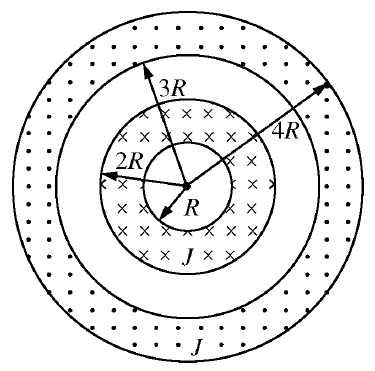
\includegraphics[scale=0.7]{images/19.png}
\end{figure}

% Multiple Choice Question 19
\begin{questions}\setcounter{question}{18}\question
Two long, hollow, concentric conducting cylinders carry currents in opposite directions into and out of the plane of the page, as shown in the cross section above. The currents are unequal, but the current density $J$ is the same for both cylinders. In which of the following regions can the net magnetic field be zero at some nonzero finite distance $r$ from the central axis?

\begin{choices}
\choice $r<R$ only
\choice Both $r<R$ and $R<r<2 R$
\choice Both $r<R$ and $2 R<r<3 R$
\choice Both $r<R$ and $3 R<r<4 R$
\choice $r>4 R$ only
\end{choices}\end{questions}
